\documentclass{acmconf}
\usepackage{amssymb}
\usepackage{amsmath}
\usepackage{amstext}
\usepackage{proof}
\usepackage{code}
\usepackage{epsfig}
\usepackage{color}
\usepackage{pstricks,pst-node,pst-tree}

\newcommand{\mygray}{\color{green}}
\newcommand{\mygreen}{\color{green}}

\newcommand{\bangforbindingcolon}{\mathcode`!="003A}
\bangforbindingcolon
\def\sig{\mathsf{sig}}
\def\ctx{\mathsf{ctx}}
\def\kind{\mathsf{kind}}
\def\typeb{\mathsf{type}}
\newcommand{\figfoot}{\vspace{1ex}\hrule}
\newcommand{\fighead}{\hrule\vspace{1.5ex}}

\newcommand{\z}{\mbox{}}

\newcommand{\typeLF}{\textsf{type}}
\newcommand{\propLF}{\textsf{prop}}

\newcommand{\false}{\textsf{false}}
\newcommand{\true}{\textsf{true}}
\newcommand{\andLF}{\; \textsf{and}\;}
\newcommand{\impLF}{\;\textsf{imp}\;}
\newcommand{\forallLF}{\;\textsf{forall}\;}
\newcommand{\existsLF}{\;\textsf{exists}\;}
\newcommand{\eqLF}{\;\textsf{eq}\;}
\newcommand{\eqilLF}{\;\textsf{eqi1}\;}
\newcommand{\eqirLF}{\;\textsf{eqi2}\;}
\newcommand{\eqalLF}{\;\textsf{eqa1}\;}
\newcommand{\eqarLF}{\;\textsf{eqa2}\;}

\newcommand{\orl}{\vee}
\newcommand{\andl}{\wedge}
\newcommand{\impl}{\supset}
\newcommand{\ldot}{.\,}
\newcommand{\unif}{\;\doteq\;}

%\newcommand{\andI}{\textsf{andI}}
%\newcommand{\andEL}{\textsf{andE}$_1$}
%\newcommand{\andER}{\textsf{andE}$_2$}
%\newcommand{\impI}{\textsf{impI}}
%\newcommand{\allI}{\textsf{allI}}
%\newcommand{\allE}{\textsf{allE}}
%\newcommand{\orIR}{\textsf{orI}$_1$}
%\newcommand{\orIL}{\textsf{orI}$_2$}
%\newcommand{\orE}{\textsf{orE}}
%\newcommand{\exI}{\textsf{exI}}
%\newcommand{\exE}{\textsf{exE}}
%\newcommand{\impE}{\textsf{impE}}
%\newcommand{\ax}{\textsf{axiom}}
%\newcommand{\trueI}{\textsf{trueI}}
%\newcommand{\falseE}{\textsf{falseE}}

\newcommand{\listd}{\mathsf{list }}
\newcommand{\chars}{\mathsf{char}\;}
\newcommand{\integer}{\mathsf{int}\;}
\newcommand{\nil}{\mathsf{nil}}
\newcommand{\conc}{\;;\;}
\newcommand{\cons}{\mathsf{cons }\;}

\newcommand{\vd}{\vdash}
\newcommand{\vdN}{\Vdash}
\newcommand{\arrow}{\rightarrow}
\newcommand{\hastype}{\mathrel{:}}
\newcommand{\oftp}{\mathord{:}}
\newcommand{\ofvd}{\mathord{::}}
\newcommand{\lam}{\lambda}
\newcommand{\turn}{\mathord{\scriptstyle \vdash}}

\newcommand{\ednote}[1]{\footnote{\it #1}}
\newenvironment{note}{\begin{quote}\message{note!}\it}{\end{quote}}

\newcommand{\lbb}{{[\![}}
\newcommand{\rbb}{{]\!]}}
\newcommand{\Mu}{\lbb M/u\rbb}
\newcommand{\id}{\mathsf{id}}
\newcommand{\msub}[1]{\lbb #1 \rbb}
\newcommand{\inv}[1]{{#1}^{-1}\,}

\newcommand{\type}{\mathsf{type}}
\newcommand{\mctx}{\;\mathsf{mctx}}

\newcommand{\bnfas}{\mathrel{::=}}
\newcommand{\bnfalt}{\mathrel{|}}

\begin{document}
\title{Generating and checking small proof witness for the logical
  framework LF}
\author{Susmit Sarkar and Brigitte Pientka}
\affiliation{}

\maketitle 

\abstract{Certified code systems demand the production of small-sized
objects which can witness proofs in a machine-verifiable manner. We
present a proof compression and verification engine for the logical
framework LF. This extends ideas previous work by Necula and
Rahul~\cite{necula+:oracles} in two main ways: 1) We consider the full
fragment of LF 2) We will incorporate caching of sub-proofs to
generate even more compact proof representations. This demonstrates
that many of the restrictions 

Our system is integrated into the Twelf system, which has been widely
used for certified code systems, and a wide range of experimental
results demonstrates the practicality and usefulness of proof
compression within logical frameworks.}

\section{Introduction}
Proof-carrying code applications establish trust by verifying
compliance of the code with a given safety and security policy.
A code producer verifies that the program is safe to
run according to some predetermined safety policy, and supplies a
binary executable together with its safety proof. Before
executing the program, the code consumer then quickly checks the code's
safety proof against the binary. 

Many proof-carrying code projects, in particular in foundational PCC,
have employed the logical framework LF as a general safety
infrastructure for encoding safety polcies and representing safety
proofs\cite{AppelFelty00,Crary:POPL03,AppelFelten99,Crary:CADE03}.
The main advantage of using a logical framework is its flexibility
and its smal trusted computing base. Hence, it reduces the effort
required for each particular safety policy. However, proofs within the
logical framework may be large in size 
% several mega-bytes - with LFi few tens of kilobytes (=two orders of
% magnitude) 
, e.g. 4-times as big as the
actual machine code. This has spawned a number of research
contributions to reduce proof size and proof checking time for
proof-carrying code applications. However, all these contributions
trade the expressive power and complexitity of LF against
simplicitiy. 
In a first step, Necula and Lee's \cite{Necula98lics} developed a
proof representation for LF$_i$, essentially a restriction to 2-level
logical framework, which eliminated many implicit type information in
the representation of proofs. However, proofs in LF$_i$ are still
4-times as big as the program they are certifying.
To obtain even smaller proofs (1/8th the size of the machine code),
Necula proposed in \cite{Necula+01:oracle} to only record the
non-deterministic choices which were made when constructing the proof,
and then use a guided prover to reconstruct the proof on the consumer
side. This simple idea has been proven to be effective in many
practical examples, and most recently has been proposed within the
Open Verifier Framework \cite{Necula}. Appel et al. use a similar idea
for creating a foundational proof checker with small
witnesses. However, all these approaches are restricted to simply 
typed Prolog-like engines which work on the fragment of hereditary
harrop formulas. Although thses approaches allow dynamic assumptions,
this is only one dimension in higher-order logic programming. The
other dimension, namely enriching the term language to allow terms
defined by $\lambda$-abstraction  to support encodings using higher-order
abstract syntax is usually not accounted for in practice. The reason
is two-folded: First, in simple safety policies about typed-assembly
language, higher-order abstract syntax is rarely used. However, as we
move to more complex safety policies, support for higher-order
abstract syntax will become more desirable. Second, techniques needed
to extend oracle-based proof compression and proof re-construction for
higher-order terms have been 

This is
unfortunate since higher-order features, which are often used when
encoding safety logics and type systems, need to be encoded or
circumvented using tricks or are simply disallowed. As we move beyond
proving memory safety, we predict that richer safety logics and type
systems which benefit from the full power provided by LF will play a
more important role in proof-carrying code applications. Hence the
need for general purpose proof-checkers for full LF will grow.

Moreover, as we move towards a general environment for rapid
prototyping and experimenting with a wide range of safety and security
policies for proof-carrying code applications, which may incorporate
sophisticated theorem proving technology, proof compression and proof
checking via guided proof re-construction can provide a quick valuable
soundness check. This is important to eliminate bugs. It is much faster to
proof-check via guided proof re-construction than type checking
explicit proof terms.  

In this paper, we describe the design of a oracle-based proof checker for
full LF. This demonstrates that many of the existing restrictions
which are placed on oracle-based proof checkers are unnecessary. The
main obstacle in building a oracle-based proof checker for full LF
is due to higher-order terms (e.g. terms my contain
$\lambda$-abstraction). As a consequence, known oracle-based proof checking
systems entirely avoid this problem and concentrate on the first-order
fragment, where for example unification is decidable and easily
implemented and efficient term indexing operations are known to make
it practical. In this paper, we show that this restriction to
first-order terms is unnecessary. Moreover we demonstrate it is
possible to extend Twelf with making it unnecessary to build seperate
proof checking engines.
We propose the use of higher-order substitution tree indexing together
with linear higher-order pattern unification to extend oracle-based
proof checking to the higher-order setting. Furthermore, we improve on
the size of oracle-proofs by factoring out common
sub-proofs\footnote{Eliminating common sub-proofs is an orthogonal
  problem to eliminating redundant implicit type 
  information, as is   proposed in \cite{Necula98lics}.} by
incorporating memoization techniques. Identifying and factoring out
common sub-proofs leads to more compact oracles and can  
decrease proof-checking time by a factor of ?? since common sub-proofs
are only checked once.  

We hope this will provide a comprehensive guide for future
implementations of proof checkers which need not be restricted to
first-order prolog-like systems. In particular, various
certified code systems can exploit this idea. However, small proof
witnesses not only play a role in certifiyng code, but are useful and
sometimes necessary in building in certifying theorem proving and
logic programming engines. First, constructing and possibly storing
full proof terms is expensive, considering the fact that the size of
the proof term can be at least 4-times as big as the statement we are
trying to prove. Hence witnesses provide a cheap
simple alternative. As an example consider tabled higher-order logic
programming, where we memoize subgoals together with their answers and
proofs to re-use the results later. Constructing and storing the full
proof term however would impose a substantial performance
penalty. Hence, small witnesses in forms of oracles  provide a cheap
simple alternative and are in fact crucial to obtain a practical
tabled logic programming interpreter. Second, there has been interest
in producing proof justifiers in the logic programming community to
ease debugging. Small proof witnesses can be viewed as proof
justifiers and may be used to re-trace the proof. We have implemented
a oracle-based proof generator and checker as part of the logical
framework {\em Twelf}.  

The paper is structured as follows. We give background on
higher-order logic programming in Twelf in Section~\ref{sec:twelf}. In
Section~\ref{sec:oracles}, we present our approach to oracle-based
proof generation and proof checking. In particular, we explain
higher-order term indexing to index higher-order logic programming
clauses. In Section~\ref{sec:tabling}, we discuss memoization techniques for
factoring out common subproofs. We conclude with a discussion of some
experimental results within Twelf and discussion of related work.

\section{Higher-order logic programming}\label{sec:twelf}

Higher-order logic programming extends first-order logic programming
in three main ways: First, first-order terms are replaced with
(dependently) typed $\lambda$-terms. Second, the body of clauses may
contain implications and universal quantification, thereby generating
dynamic assumptions which may be used during proof search. Thirdly,
execution of a query will not only produce a yes or no answer, but
generates a proof term as a certificate which can be checked
independently. These features make higher-order logic programming an
ideal generic framework for implementing formal safety policies given via
axioms and inference rules and executing them.

The theoretical foundation underlying higher-order logic programming
within Twelf is the LF type theory, a dependently typed lambda
calculus. We will first give an example of encoding the natural
deduction calculus in the logical framework LF using higher-order
logic programming following the methodology in \cite{harper+:lf}. For
more information on how to encode formal systems in LF see
\cite{Pfenning97}. 

Using this example, we will explain oracle-based proof generation and
proof-checking. 

\subsection{Representing Logics}
As a running example, we will consider intuitionistic logic formulated
in the natural deduction style. We will only concentrate on the fragment
consisting of implications and universal quantifiers. Propositions can
be then described as followsL
\[
\begin{array}{llll}
\mbox{Propositions} & A,B, C & := & \top \mid A \impl B \mid \forall x.A \\
\mbox{Context} & \Gamma & := & \ldot \mid \Gamma,  A
\end{array}
\]

Inference rules describing natural deduction are presented in Table~\ref{natded}.

\begin{table}[h]
\fighead
\[
\infer{\Gamma\vdash \forall x. A}
{\Gamma\vdash [a/x]A & a \mbox{ is new}}
\qquad
\infer{\Gamma\vdash [T/x]A}
{\Gamma\vdash \forall x.A}
\]
\[
\infer{\Gamma\vdash A\impl B}
{\Gamma,A\vdash B}
\qquad
\infer{\Gamma\vdash B}
{\Gamma\vdash A\impl B
\quad
\Gamma\vdash A}
\]
%\[
%\infer{\Gamma\vdash A\andl B}
%{\Gamma\vdash A\quad \Gamma\vdash B}
%\qquad
%\infer{\Gamma\vdash A}
%{\Gamma\vdash A\andl B}
%\qquad
%\infer{\Gamma\vdash B}
%{\Gamma\vdash A\andl B}
%\]
%\[
%\infer{\Gamma\vdash A\orl B}
%{\Gamma\vdash A}
%\qquad
%\infer{\Gamma\vdash A\orl B}
%{\Gamma\vdash B}
%\]
%\[
%\infer{\Gamma\vdash C}
%{\Gamma\vdash A\orl B
%\quad
%\Gamma,A\vdash C
%\quad
%\Gamma,B\vdash C
%}
%\]
\[
\infer{\Gamma\vdash\top}
{}
\qquad
\infer{\Gamma\vdash C}
{\Gamma\vdash\perp}
\qquad
\infer{\Gamma, A \vdash A}
{}
\]
\caption{\label{natded}A natural deduction system}
\figfoot
\end{table}

To represent this system in LF, we first need formation rules to
construct terms for the objects we are talking about, in this case,
propositions. We declare a new type {\tt prop} for propositions and a
type {\tt i} for individuals. We intend that terms belonging to {\tt
  prop} represent well-formed propositions. The rules are given below,
in concrete Twelf syntax. 

\begin{code}
prop : type.
i    : type.
\vspace{0.1in}
true   : prop.
false  : prop.
imp    : prop -> prop -> prop.
forall : (i -> prop) -> prop.
\end{code}

The connectives for implication takes in two propositions and returns a
proposition. To represent the forall-quantifier, we will use
higher-order abstract syntax. The crucial idea is to represent bound
variables in the object language (logic) with bound variables in the
meta-language (higher-order logic programming). 

Next we turn our attention to the proofs in our system. We have a
judgment for provability within this logic. We map this judgment to
a type family {\tt prov}, which has a (dependent) kind.

\begin{code}
prov : prop -> type.
\end{code}

Each clause will correspond to an inference rule in the object
logic. For convenience, we give the constructors 
descriptive names, and follow the order of the rules in
Table~\ref{natded}. 

\begin{code}
alli   : prov (forall $\lambda$x. A x)
            <- $\Pi$x. prov (A x)
alle   : prov (A T)
            <- prov (forall $\lambda$x. A x).
\z
impi     : prov (imp A B)
            <- (prov A -> prov B).
impe     : prov B
            <- prov (imp A B)
            <- prov A.
\end{code}

%\z
%truei    : prov true.
%\z
%falsee   : prov C
%            <- prov false.

These rules are given as a Twelf signature. $A$, $B$, $C$ denote
existential or logic variables which are instantiated during proof
search.  
There are two key ideas which make the encoding of the sequent
calculus elegant and direct. First, we use the power of dynamic
assumptions which higher-order logic programming provides, to
eliminate the need to manage assumptions in a list explicitely. To
illustrate, we consider the clause {\tt impI}. To  prove {\tt prov (A
  => B)}, we prove {\tt prov B} assuming {\tt prov A} In other words,
the proof for $prov B$ may use the dynamic assumption $prov A$. 

Second, we use higher-order abstract syntax to encode the bound
variables in the universal quantifier. As a consequence substitution
in the object language can be reduced to application and
$\beta$-reduction in the meta-language (higher-order logic
programmining). Consider the rule for all-elimination. If we have a proof of
$\forall x.A$ , then we know that $[T/x]A$ is true for any term
$T$. The substitution $[T/x]A$ in the object language is achieved via
application in the meta-language {\tt A T}. 



\subsection{Proof search in higher-order logic programming}

Higher-order logic programming is similar to a Prolog interpreter
since it performs essentially a depth-first search over all the
program clauses. However, in the higher-order setting we may have
dynamic assumptions which may be used within a certain
scope. Moreover, since Twelf allows higher-order terms (i.e. terms may
contain $\lambda$-abstraction), higher-order unification is used to
unify clause heads with current goal. Finally, proof terms are
generated.

We will illustrate proof search by considering the following example: {\tt prov (forall $\lambda$y. (imp (forall $\lambda$ x. P x) (P y)))}
(corresponding to $(\forall y. (\forall x.P(x)) \impl P(y)$).  The
proof tree for this is shown in Figure~\ref{prooftree1}.

\begin{figure}
\fighead
\epsfig{file=prooftree1.ps,width=2.7in}
\caption{\label{prooftree1} Proof Tree for 
$\top\impl((\top\impl\perp)\impl\perp)$}
\figfoot
\end{figure}
      
We first start with trying to prove {\tt prov (forall $\lambda$y. (imp
  (forall $\lambda$ x. P x) (P y)))}. This means at least three
clause heads will unify with the current goal, namely {\tt alli}, {\tt
  impe} and {\tt impe}. We pick the first of these applicable clauses ({\tt
alli}). This will yield the next subgoal {\tt $\Pi$ y. prov (imp
(forall $\lambda$ x. P x) (P y))}. This means we need to show for any
{\tt y}, that {\tt prov (imp (forall $\lambda$ x. P x) (P y))} is true.
To prove {\tt prov (imp (forall $\lambda$ x. P x) (P y))} for any
parameter {\tt y}, will again inspect our clauses. Three of them will
be applicable, namely {\tt alle}, {\tt impi}, and {\tt impe}. This
time we will pick the second clause {\tt impi}. Hence we will
introduce the dynamic assumption {\tt u : prov (forall $\lambda$ x. P x)}
and show {\tt prov (P y)} using this assumption. In the third step,
again two clauses are applicable,  {\tt alle}, and {\tt
  impe}. Using the first one, {\tt alle}, we need to show that we can
prove {\tt prov (forall $\lambda$ x. P x)}. There are in fact 4
possible clauses whose will clause head will unify: the dynamic clause
{\tt u} and the three program clauses {\tt alli}, {\tt alle}, and {\tt
  impe}. Using 
the dynamic assumption {\tt u}, we can finish the proof. The final
proof term which will be generated by Twelf's higher-order logic
programming engine is : 

{\tt (alli $\lambda$ y. (impi $\lambda$ u. (alle y u)))}.

 From an operational view point, the search can be described as
 follows: 

\begin{table}[htbp]
\fighead
\begin{small}
Solve Goal $\Gamma \vd M : G$:
\begin{enumerate}
\item $\Gamma \vd (c \cdot S) : G$ \\
    \mbox{Given an atomic goal $G$ and clauses $\Gamma$:}\hfill\\
     Focus on a clauses $c : A$ from $\Gamma$ to establish a proof $S$ for $G$.

\item $\Gamma \vd \lambda u.M : G_1 \arrow G_2$ if $\Gamma, u\oftp G_1
  \vd M : G_2$ \\
Augment the clauses in $\Gamma$ with the dynamic assumption $u : G_1$ and
establish a proof $M$for the goal $G_2$ from the extended  program $\Gamma, u \oftp G_1$.
\item $\Gamma \vd \lambda a.M : \Pi x. G$ if $\Gamma \vd M : [a/x]G$ where $a$ is a new parameter\\
Given a universally quantified goal $\Pi x. G$, we
generate a new parameter $c$, and establish a proof $M$ for $[c/x]G$ in the
 program context $\Gamma$.
\end{enumerate}
\end{small}
\figfoot 
\caption{Solve goal $G$ from clauses in $\Gamma$}
\label{tab:solve}
\end{table}

Once the goal is atomic, we need to select a clause from the
program context $\Gamma$ to establish a proof for $G$. In a logic
program interpreter, we consider all the clauses in $\Gamma$ in order. 
First, we will consider the dynamic assumptions, and then we will try
the static program clauses one after the other. 
Let us assume, we picked a clause $A$ from the program context
$\Gamma$ and we now need to establish a proof for $G$.

\begin{table}[h]
\fighead
\begin{small}
Focus on clause $ c : A$ to solve atomic goal $P$.
\begin{enumerate}
\item $\Gamma > P' \vd \nil : P$ \\
 Given the atomic clause $P'$ with name $n$, we establish a proof for the
  atomic goal $P$, by checking  $P' = P$. If yes then
  succeed. Otherwise fail and backtrack.  
\item $\Gamma > n : G_2 \arrow G_1 \vd (M ; S) : P$ 
      if $\Gamma > G_1 \vd S : P$ and  $\Gamma \vd M : G_2$ \\
  Given the clause $G_2 \arrow G_1$ with name $n$, we establish a
  proof of the atomic goal $P$, by trying to use the clause $G_1$ to
  establish a proof $M$ for $P$. If it succeeds, we establish a proof
  $S$ for the goal $G_2$. If it fails,  backtrack. 
\item $\Gamma > n : \Pi x\oftp A_1. A_2 \vd S : P$ if $\Gamma > n :
  [T/x]A_2 \vd (T ; S) : P$\\
  Given the clause $\Pi x\oftp A_1. A_2$ with name $n$, we
  establish a proof $(T ; S)$for the atomic goal $P$ by instantiating
  $x$ with a term $T$, and use the clause $[T/x]A_2$
  to establish a proof $S$ for the atomic goal $P$. 
\end{enumerate}
\end{small}
\figfoot
  \caption{Focus on clause $c:A$ to solve atomic goal $P$}
  \label{tab:foc}
\end{table}


Typically a logic programming interpreter needs to resolve two
choices. The first choice lies in picking the correct instantiation
$T$ in foc-step 3. Typically, we introduce logic (or existential) variables in step
3, which will then be instantiated during unification in foc-step 1 to
eliminate existential-nondeterminism. Although in first-order setting,
this is decidable, in the higher-order setting this is more
difficult. The second choice lies in solv-step 1 of solving a goal,
where we need to pick the correct program clause from
$\Gamma$. Usually, we will try the clauses in order, starting with the
dynamic clause and then continuing with the static program
clauses. However, as we saw in the previous example, there are several
possible candidates, and usually only one of them is fruitful to
pursue. Note that during proof search we typically have the program
clauses $\Gamma$ and the goal $G$ we are trying to prove from the
clauses in $\Gamma$ as inputs, while the proof term $M$ is the output
of the search.

 Our goal is to reduce the proof evidence to the
non-deterministic choices we have made during the proof to produce
small proof witnesses.  
      
\section{Oracle-based proof search}
\label{sec:oracles}

In this section, we describe the oracle-based proof generation and
checking. To generate oracles we can follow two ways. First, we may
modify the logic-programming proof search procedure available to generate
a bit-string during proof search directly. As in general logic
programming's depth-forst search is incomplete, this may not work
general, although it can be often done with more sophisticated theorem
proving  technology. In certifying code systems however the safety proof is
usually generated by a certifying compiler, and we merely aim at
compressing the safety proof into a bit-string. In the latter case, we
pass into the described search procedure, the program clauses
$\Gamma$, the goal $G$ and the proof term $M$. This way, we can
eliminate all non-determinism from the previous search procedure.

\subsection{Generating small proof witnesses}

In this section, we will describe the modifications needed to generate
a compact proof witness in form of a bit-string using the verifier's
proof search procedure from the previous section. The bit-string
encodes the non-deterministic choice within the proof. As outlined in
the previous section, there are two different kinds of choices: 1)
Existential choice which is resolved via higher-order pattern
unification and 2) picking the right clause $c$ from the
program context $\Gamma$ to establish a proof $S$ for $P$, once the
goal $P$ is atomic. Potentially, there is more than one clause whose head
unifies with $P$, and hence a proof search procedure needs to consider
all the possible choices in order.  

The key insight for generating a compact proof wtness is that proof
search is deterministic, if we know what program clause or dynamic
clause to pick for each subgoal (see the procedure for solving goal
$A$ from clauses in $\Gamma$, step 1). Let us briefly consider the
previous example to illustrate. To prove

\[
(\forall y. (\forall x.P(x)) \impl P(y)
\]

A prover must consider the following choices: At the top level, we
have to prove a universal quantifer and 3 choices apply ({\tt alli},
{\tt impe}, and {\tt impe}), and we took the first one. At the next
stage, again 3 choices apply, namely {\tt alle}, {\tt   impi}, and
{\tt impe}. In the third stage, we have two applicable clauses, {\tt
  alle}, and {\tt impe}, and in the final step we have four potential
candidates. Note that at each stage the proof term {\tt (alli
  $\lambda$ y. (impi $\lambda$ u. (alle y u)))} tells us exacly which
choice to focus on.

This process eventually finds the proof. The list of
choices made in this proof search procedure is $1/3$, $2/3$, $1/2$,
$1/4$, keeping in mind that dynamic assumptions are tried first by
proof search procedures. This sequence will constitute our compact
proof witness and is all that needs to be generated and sent to the
verifier.  

This leads to an efficient encoding of the choices. If we have $k$
choices, we need $\lceil\log_2 k\rceil$ bits. Since we know that the
path through the proof tree always has to lead to a proof, if there is
only one choice applying, this formula correctly says that we do not
need to emit an advice.  The verifier knows how many choices apply, so
she can calculate the number of bits to pick off the oracle. This
means that we do not need an explicit separator between the choices,
although we include them here for better readability.
The witness corresponding to the non-deterministic choices in the
previous example is: {\tt 100010101000}.

For the idea to work, proof witness generation and witness checking
have to perform essentially the same overall proof search. Moreover,
the order in which different choices are considered must be the same.
The only difference is that during witness generation we would explore
possible multiple fruitless paths until settling on the right one,
while in witness checking we know by inspecting the advice encoded in
the bit-string which choice to consider.

The oracle-string encodes one type of possible choices, but as we
briefly mentioned earlier, unification in the higher-order setting is
undecidable in general. In Twelf, we use a higher-order pattern
unification algorithm together with constraints. Higher-order pattern
unification is in fact decidable.Although it is too restrictive to
concentrate solely on higher-order patterns statically, 
most of the non-patterns encountered (for example $(A\;T)$), will be a
pattern during execution. Since we assume that we already found a proof $M$
for a goal $G$ without any left-over unification constraints, 
all the unification problems solved during execution were
decidable. It is worth pointing out that our proposal differs here
from the proposal of Necula and Rahul, who propose to encode the
non-deterministic choice of Huet's unification algorithm, which does
not distinguish between higher-order patterns and non-patterns. 

\subsection{Checking small proof witnesses}
In this section, we modify the previous search procedure, in such a
way that it is not parameterized by the proof term $M$, but rather by
the compact proof witness encoded as a bit-string. Therefore we have :

\begin{center}
Solve Goal $\Gamma \vd W : G$, where $W$ is a compact proof witness.  
\end{center}

So in step $solv-1$, we first generate the $n$ possible candidates which
will unify with the current goal $G$. If $n$ is greater than 1, we
will take off $n$ bits from the witness. If a bit $1$ occurs at
position $p$ of these $n$ bits, we will pick the $p$-th candidate.

To check that proof witnesses in fact constitute a valid proof for a
given proposition, we re-run the prover guided with the advice encoded
in the bit-string. The witness checker is then in fact a deterministic
search procedure. No backtracking is necessary, since all the
non-deterministic choices are resolved.  By taking the appropriate
branches (and performing the needed substitutions of universal
variables by unification), the user can be convinced that such a
proof exists. This can lead to savings of time and memory.
This however requires the code consumer to trust the witness
checker -- which includes trusting higher-order pattern
unification. For a paranoid consumer this may be unacceptable since
the witness checker may use optimizations such as caching subproofs
and indexing, which can be quite complicated. In this case, it is
possible to also decompress the proof witness to an explicit proof
term and use a different trusted type-checker to verify the expanded
proof witness. 

\section{Optimizations: Higher-order Term Indexing}

A proof search procedure must have a way of retrieving all clauses of
the logic program which may satisfy the current goal, since such a
method will dictate how many choices we are returned at any step, and
hence is critical in understanding the oracle. Most first-order logic
programming interpreter use term indexing strategies to efficiently
retrieve all clauses whose head unifies with the current goal.

In the higher-order setting, much fewer indexing strategies exist for
higher-order terms and are not generally known. For the purpose of
this paper, we will adopt higher-order substitution trees as described
in \cite{Pientka:ICLP03}.Substitution tree indexing has been
successfully used in a first-order setting \cite{graf:substtrees} and
allows the sharing of common sub-expressions via substitutions. This
is unlike other non-adaptive term indexing, which only allow sharing
of common term prefixes. Moreover, the technique is sound and complete
for linear higher-order patterns.

To appreciate the difficulties in higher-order term indexing and
understand why all existing witness generation and checking procedures
avoid it, we briefly summarieze the main challenges:
 First of all, building a substitution tree relies on computing the
 most specific generalization of two terms. However in the
 higher-order setting, the most specific generalization of two terms (heads)
 does not exist in general. Second, retrieving all heads, which unify
 with the current goal, needs to be efficient --
but higher-order unification is undecidable in general.  As discovered
by Miller \cite{Miller91iclp}, there exists a decidable fragment,
called higher-order patterns. For this fragment, unification and
computing the most specific generalization is decidable even in 
rich type theories with dependent types and polymorphism as shown by
Pfenning \cite{Pfenning91lics}.  However, these algorithms may not be
efficient in practice  \cite{PientkaPfenning:CADE03} and hence it is
not obvious that they are suitable for higher-order term
indexing techniques. 

In \cite{Pientka:ICLP02}, we propose substitution tree indexing for
higher-order terms based on linear higher-order patterns. Linear
higher-order patterns refine the notion of higher-order patterns
further and factor out any computationally expensive parts. As shown
in \cite{PientkaPfenning:CADE03}, many terms encountered fall into
this fragment and linear higher-order pattern unification performs well in
practice. In \cite{Pientka:ICLP02,Pientka:Phd}, we give a formal
description for computing the most specific generalization of two
linear higher-order patterns, for inserting terms in the index and for
retrieving a set of terms from the index s.t. the query is an instance
of the term in the index, and show correctness. This can be extended
to unifiability. For this setup to work cleanly in the higher-order
setting, it is crucial that we distinguish between existential
variables in $\Delta$ and bound variables and assumptions in
$\Gamma$. Moreover, it is essential that existential variables allow
in place up-date. In particular, we will rely on the notion of
existential variables which are ``fully applied'', i.e. they may
depend on all the bound variables they occur in.

 In the following, we will describe requirements and
challenges we face of memoizing sub-goals in the higher-order setting. 


\[
\begin{array}{ll}
\eqLF: & \propLF \rightarrow \propLF \rightarrow \typeLF.\\[1em]
%
\eqilLF: & \eqLF (\forallLF \lambda x. \impLF (A\; x)\; B)\quad (\impLF (\existsLF \lambda x. A\; x)\; B).\\
\eqirLF: & \eqLF (\forallLF \lambda x. \impLF A \; (B\; x)) \quad (\impLF A\; (\forallLF \lambda x. B\;x)).\\
\eqalLF: & \eqLF (\forallLF \lambda x. \andLF (A\; x)\; B) \quad (\andLF (\forallLF \lambda x. A \;x) \; B).\\
\eqarLF: & \eqLF (\forallLF \lambda x. \andLF A \; (B\;x)) \quad (\andLF A \; (\forallLF \lambda x. B\; x)).\\
\end{array}
\]

After linearization:
\[
\begin{array}{ll}
\eqLF: & \propLF \rightarrow \propLF \rightarrow \typeLF.\\[1em]
%
\eqilLF: & \eqLF (\forallLF \lambda x. \impLF (A'\; x)\; (B'\;x)\quad (\impLF (\existsLF \lambda x. A\; x)\; B). \\
         & \forall x. (A'\; x) \unif (A \; x) {\textsf{ and } } B'\;x   \unif B\\[0.5em]
\eqirLF: & \eqLF (\forallLF \lambda x. \impLF (A'\;x) \; (B'\; x)) \quad (\impLF A\; (\forallLF \lambda x. B\;x)).\\
         & \forall x. (A'\; x) \unif A  {\textsf{ and }} B'\;x   \unif (B\;x)\\[0.5em]
\eqalLF: & \eqLF (\forallLF \lambda x. \andLF (A'\; x) \; (B'\;x)) \quad (\andLF (\forallLF \lambda x. A \;x) \; B).\\
         & \forall x. (A'\; x) \unif (A \; x) {\textsf{ and }} B'\;x   \unif B\\[0.5em]
\eqarLF: & \eqLF (\forallLF \lambda x. \andLF (A'\;x) \; (B' x)) \quad (\andLF A \; (\forallLF \lambda x. B\; x)).\\
         & \forall x. (A'\; x) \unif A  {\textsf{ and }} B'\;x   \unif (B\;x)\\[0.5em]
\end{array}
\]


%
% eqi1: eq (forall $\lambda$ x. imp (A' x) (B' x)) (imp (exists $\lambda$ x. A x) B).
% residual equations: B' x = B    A' x = A x

% eqi2: eq (forall $\lambda$ x. imp (A' x)  (B' x)) (imp A (forall $\lambda$ x. B x)).
% residual equations: B' x = B x    A' x = A

% eqa1: eq (forall $\lambda$ x. and (A' x)  (B' x)) (and (forall $\lambda$ x. A x) B).
% residual equations : A' x = A x   B' x = B

% eqa1: eq (forall $\lambda$ x. and (A' x)  (B' x)) (and A (forall $\lambda$ x. B x)).
% residual equations: B' x = B x    A' x = A
%
%
%
%
% \begin{small}
\begin{figure*}[htbp]
  \begin{center}
    \begin{small}
\pstree[nodesep=1pt,levelsep=9ex]{%
\TR{$\eqLF (\forallLF \lambda x. i_1[\id]) \quad i_2[\id]$} }{%
  \pstree{\TR{\begin{tabular}{r}
              $(\andLF A'[\id]\; B'[\id])/i_1$\\
              $(\andLF i_3[\id]\; i_4[\id])/i_1$\\
            \end{tabular}
          }
        }{%
          \pstree{\TR{\begin{tabular}{r}
                $\forallLF \lambda x. A[\id]/i_3$,\\
                $B/i_4$
              \end{tabular}
            }}{%
            \pstree{\TR{\begin{tabular}{l}
                  $A'[\id]\unif A[x/x]$\\
                  $B'[\id]\unif B$
                \end{tabular}
              }}{ $\eqarLF$}
          }
%
          \pstree{\TR{\begin{tabular}{r}
                $A/i_3,$\\
                $\forallLF \lambda x.B[\id]/i_4$
              \end{tabular}
            }
          }{%
            \pstree{\TR{\begin{tabular}{l}
                $A'[\id]\unif A$\\
                $B'[\id] \unif B[\id]$
              \end{tabular}
            }
            }{ $\eqalLF$}
          }
        }
%%%%% second child
          \pstree{\TR{\begin{tabular}{r}
                     $(\impLF A'[\id]\; B'[\id])/i_1$\\
                     $(\impLF i_3[\id]\; i_4[\id])/i_2$\\
                   \end{tabular}
                 }}{
                 \pstree{\TR{\begin{tabular}{r}
                       $\forallLF \lambda x. A[\id]/i_3$,\\
                       $B/i_4$
                       \end{tabular}
                     } }{%
                     \pstree{\TR{\begin{tabular}{l}
                           $A'[\id]\unif A[x/x]$\\
                           $B'[\id]\unif B$
                         \end{tabular}}
                     }{$\eqirLF$}
                   }
                  \pstree{\TR{\begin{tabular}{r}
                        $A/i_3,$\\
                        $\forallLF \lambda x.B[\id]/i_4$
                      \end{tabular}}}{
                    \pstree{\TR{\begin{tabular}{l}
                          $A'[\id]\unif A$\\
                          $B'[\id] \unif B[\id]$
                        \end{tabular}}
                    }{$\eqilLF$}
                  }
                }
              }
        
    \end{small}
  \end{center}
  \caption{Substitution tree}
  \label{fig:substree}
\end{figure*}

% \end{small}

In contrast to other indexing techniques such as discrimination tries,
substitution trees  allows the sharing of common sub-expressions
instead of common term prefixes.

This is especially important for indexing dependently typed terms. 

\begin{note}
  Give an example? -- for example, annotate every formula with its size?
\end{note}

We have chosen to index only the static set of program clauses. In
theory, it is possible to use substitution tree indexing for dynamic
clauses generated during proof search.  However, it is not clear how
useful this will be, since the process of creating the tree itself is
time-consuming. It is also noted by Necula and Rahul \cite{} that
indexing dynamic assumptions imposes a performance penalty. It is
useful to pre-process the program, but the payoff with dynamic clauses
is unclear. For dynamic clauses, we use only simple head term matching.


\section{Caching results}
\label{sec:tabling}
Since large proofs often have identical subproofs,  there is a
lot of opportunity for sharing subproofs. The problem is particularly
acute in machine-generated proofs for certifying machine-code which
tend to have repeated proofs of simple facts. This problem has been
already pointed out by Necula and Lee in \cite{NeculaLee+97:resource}

 \begin{tabular}[h]{l}
``...it is very common for the proofs to have  \\
repeated sub-proofs that should be hoisted out and \\
proved only once ...'' \cite{NeculaLee+97:resource}\\ $\;$
 \end{tabular}


In the context of oracle-based proof checking, this leads to two
problems.  First, the oracles become larger in size than
necessary. This means that what has to be transmitted to the verifier
is large in size. Secondly, the performance of witness checker may
degrade, since it spends its time uselessly proving the same fact over
and over again. 

Ideally we would like to cache intermediate results and re-use them
later. Up to now, this has been difficult since we need to efficiently
store and retrieve intermediate goals. We re-use and build upon recent
work \cite{pientka:tabled} on memoizing intermediate goals during
execution as part of the tabled higher-order logic programming and
adapt it for witness generation and witness checking. 

When we generate compressed witnesses from explicit proof terms or
when we check compressed witnesses, we have the advantage that we know
a proof exists. This is simplifies memoization substantially, since we
can add the goal together with its answer substitution and proof
witness into a memo-table once we finished proving a given subgoal. 
\begin{note}
  Susmit: I can't find your code to look up how we decided to
  implement caching. Please double-check what I claim here...
\end{note}

We modify again the first step of the proof. First, we will check if there
exists already a table entry $\Gamma \vd G$ together with an answer
and proof witness in the memo-table for the current goal $\Gamma \vd
G$. If there exists no entry, such an answer we will re-use it and return the
proof witness $W$. If there is no 
Second, we will destructively update
the memo-table when we have proven a goal. In addition to returning
the proof witness $i . w$, we destructively update the memo-table, by adding the current goal
$\Gamma \vd G$ together with its answer substitution and proof witness
$i . w$.  


\begin{note}
  Say how to store elements in a table.
The table setup is as follows:
\[
\begin{array}{ll}
\mbox{Table entry} & \Delta ; \Gamma \vd G\\
\mbox{Residual Equ.} & \Delta ; \Gamma \vd R \\
\mbox{Answer substitution} & \Delta' \vd \theta : \Delta
\end{array}
\]

Apply strengthening to detect more identical subproofs (strengthening
based on subordination and on not adding dynamic assump twice)
The design supports naturally substitution factoring based on explicit
substitutions\cite{RamakrishnanJLP99}. With substitution factoring the
access cost is proportional to the size of the answer substitution
rather than the size of the answer itself\footnote{may not be necessary in
this setting -bp?}
\end{note}

The stored solution to a tabled goal is not always the solution we
want to use.  This is because using a particular answer will constrain
the free variables, possibly in ways not helpful to the proof. 

We add the choices from the table to the menu of choices available at
every choice point. Again, both the prover and verifier are following
similar algorithms, so both have identical caches. The number of
choices is also the same in both the prover and verifier. We just need
a convention on how to specify a tabled answer, and we choose the
choices appearing in the table to precede the other choices.

\begin{figure}
\fighead
\hspace{-0.5in}
\psfig{file=prooftree3.ps,width=2.7in,height=2.5in}
\vspace{1.5in}
\caption{\label{prooftree3}
$(\top\impl((\top\impl\perp)\impl\perp) \andl
(\top\impl((\top\impl\perp)\impl\perp)$}
\figfoot
\end{figure}

To take an example, look at the proposition
$(\top\impl((\top\impl\perp)\impl\perp) \andl
(\top\impl((\top\impl\perp)\impl\perp)$, whose proof tree is
given in Figure~\ref{prooftree3}. Notice the common subtrees marked
with dotted lines.  In the absence of caching results, the sequence of
choices would be 3/5, 1/5, 2/6, 3/6, 1/7, 2/6, 1/5, 2/6, 3/6, 1/7, and
2/6. With caching of results, we get the substantially shorter oracle
3/5, 1/5, 2/6, 3/6, 1/7, 2/6, and 1/6.

\section{Experimental Results}

We show an extensive experimental evaluation of the generating and
checking proofs using compact proof witnesses.

\subsection{Foundational Proof Carrying Code}
Here we consider the typed assembly language. The type system
guarantees safety.

\subsection{Sequent Calculus as a general Safety Logic}
Here we consider the sequent calculus as a general safety logic.

\subsection{Refinement Types as an advanced type system}
In this section, we consider an advanced type system based on
refinement types for a high-level ML-like language. 


\section{Related Work}
The idea of using oracles which encode the non-deterministic choice in
a logic programming interpreter was first proposed by
\cite{necula+:oracles}. Their proposal has several restriction which
our work overcomes. First, Necula and Rahul concentrate on the
fragement $LF_i$, which concentrates on 2-level fragment of
LF. They propose the use of automa-driven indexing for program
clauses, where any higher-order features are ignored. Hence their
indexing algorithm will generate a set of potential candidates, which
may include candidates which are unsound. To weed out the unsound
candidates, full higher-order unification based on Huet's algorithm is
called. This is clearly wasteful, since we will traverse higher-order
terms at least twice. In addition, their work does not consider
general terms defined via $\lambda$-abstraction. To handle some simple
cases like the {\tt alli} rule in our example, they introduce a hack
to deal with this special case.

Finally, their experimental results use a simplistic version which
concentrates on first-order unification.  In fact our work continues,
where Necula and Rahul left of ``more experimental results are needed
especially in the higher-order setting''.

Our work extends this approach to full LF by removing any of
these restriction, and incorporating higher-order term indexing as
well as caching intermediate results. There is also an important
difference in how we generate bit-strings:

\begin{note}
  Susmit: say more about the difference and why ours is better.
\end{note}


The idea of using oracles was also explored in
\cite{wu+:foundationalproofcheck}. Their primary concern was to 
achieve a minimal proof checker, in terms of number of lines of
code. Their checker is really minimal, since it follows the path
explored by Necula and Rahul and ignores higher-order
terms. The main difference is that the proof rules are proven correct
independently. Minimizing the trusted computing base is a useful
goal, but not the focus of our work. Omitting higher-order terms or
treating them in a special way, trades complexity of higher-order
unification and higher-order indexing against a specialized proof
checker for TALT. Our goal is to design a general purpose tool to
compress proofs to compact witnesses and check proofs for the logical
framework Twelf. Our work is not only useful to experiment with
proof-carrying code applications, but we also have incorporated it
into the a more sophisticated theorem prover which relies on 
redundancy elimination techniques. 


\section{Conclusion}


\bibliographystyle{plain}
\bibliography{bib}
\end{document}



